\begin{figure*}
\centering

\begin{subfigure}[b]{.15\linewidth}
  \centering
  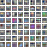
\includegraphics[width=0.9\linewidth]{figs/discrim_filters_r.png}
  \caption*{$D$}
\end{subfigure}
\begin{subfigure}[b]{.4\linewidth}
  \centering
  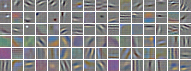
\includegraphics[width=0.9\linewidth]{figs/encoder_filters_r.png}
  \caption*{$E$}
\end{subfigure}
\begin{subfigure}[b]{.4\linewidth}
  \centering
  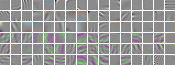
\includegraphics[width=0.9\linewidth]{figs/jigsaw_conv1_r.png}
  \caption*{\citet{jigsaw}}
\end{subfigure}

\begin{subfigure}[b]{.15\columnwidth}
  \centering
  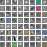
\includegraphics[width=0.9\linewidth]{figs/gen_filters_r.png}
  \caption*{$G$}
\end{subfigure}
\begin{subfigure}[b]{.4\linewidth}
  \centering
  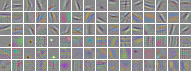
\includegraphics[width=0.9\linewidth]{figs/alexnet_discrim_conv1_r.png}
  \caption*{AlexNet-based $D$}
\end{subfigure}
\begin{subfigure}[b]{.4\linewidth}
  \centering
  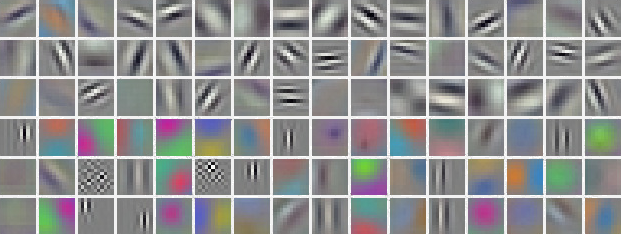
\includegraphics[width=0.9\linewidth]{figs/alexnet_conv1_r.png}
  \caption*{\citet{supervision}}
\end{subfigure}
\caption{
The convolutional filters learned by the three modules ($D$, $G$, and $E$) of a BiGAN (left, top-middle)
trained on the ImageNet~\citep{imagenet} database.
We compare with the filters learned by a discriminator $D$ trained with the same architecture (bottom-middle),
as well as the filters reported by~\citet{jigsaw},
and by~\citet{supervision} for fully supervised ImageNet training
(right).
}
\label{fig:filters}
\end{figure*}
